\Problem{Cliffside Midair Collision}{\CliffMidColl}{
You are standing at the bottom of a cliff, your friend is standing at the top, and each of you is in possession of a ball. Your friend drops the ball off of the edge, and at the exact same time, you throw your ball up toward it such that they collide in midair.
}
\Solution{\CliffMidCollSol}{

Let $h$ be the height of the cliff, $y_{c}$ be the height of the collision, $m_{d}$ be the mass of the ball your friend drops, and $m_{l}$ be the mass of the ball you launch upward. At the time of the drop and launch, $t_{i}$, your friend's ball is at rest at height $h$, and yours has initial speed $v_{li}$ at height zero. At the instant right before the collision, $t_{bc}$, both balls are at $y_{c}$, with your friend's ball moving at speed $v_{dbc}$ and your ball moving at speed $v_{lbc}$. The instant after the collision, $t_{ac}$, your friend's ball has speed $v_{dac}$, and your ball has speed $v_{lac}$. The time at which your friend's ball reaches the top of the cliff once again will be denoted $t_{f}$.

\begin{figure}[h]
	\centering
	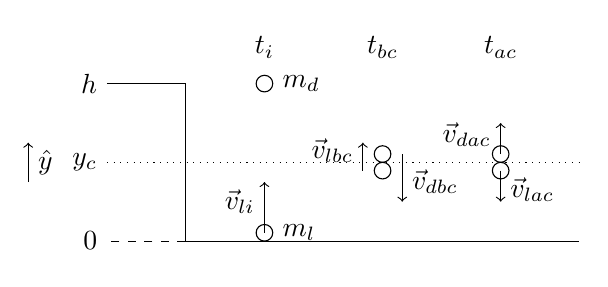
\begin{tikzpicture}
		\draw[->] (-1,0.75) -- (-1,1.25);
		\node[anchor=west] at (-1,1) {$\hat{y}$};
		\node[anchor=east] at (0,2) {$h$};
		\draw (0,2) -- (1,2) -- (1,0);
		\node[anchor=east] at (0,1) {$y_{c}$};
		\draw[dotted] (0,1) -- (6,1);
		\draw[dashed] (1,0) -- (0,0);
		\node[anchor=east] at (0,0) {$0$};
		\draw (1,0) -- (6,0);
		\node[anchor=south] at (2,2.2) {$t_{i}$};
		\draw (2,3pt) circle (3pt);
		\node[anchor=west] at (2cm+3pt,3pt) {$m_{l}$};
		\draw[->] (2,3pt) -- (2,0.75);
		\node[anchor=east] at (2,0.5) {$\vec{v}_{li}$};
		\draw (2,2) circle (3pt);
		\node[anchor=west] at (2cm+3pt,2) {$m_{d}$};
		\node[anchor=south] at (3.5,2.2) {$t_{bc}$};
		\draw (3.5,1cm-3pt) circle (3pt);
		\draw[->] (3.25,1cm-3pt) -- (3.25,1.25);
		\node[anchor=east] at (3.25,1.15) {$\vec{v}_{lbc}$};
		\draw[->] (3.75,1cm+3pt) -- (3.75,0.5);
		\node[anchor=west] at (3.75,0.75) {$\vec{v}_{dbc}$};
		\draw (3.5,1cm+3pt) circle (3pt);
		\node[anchor=south] at (5,2.2) {$t_{ac}$};
		\draw (5,1cm-3pt) circle (3pt);
		\draw (5,1cm+3pt) circle (3pt);
		\draw[->] (5,1cm+3pt) -- (5,1.5);
		\node[anchor=east] at (5,1.35) {$\vec{v}_{dac}$};
		\draw[->] (5,1cm-3pt) -- (5,0.5);
		\node[anchor=west] at (5,0.65) {$\vec{v}_{lac}$};
	\end{tikzpicture}
\end{figure}
}
\ProblemSub{\CliffMidCollA}{
(a) At what height do the two balls collide? How fast is your ball going when the two balls collide?
}
\Solution{\CliffMidCollASol}{

Based on kinematics, we know that for the dropped ball,
\[
y_{c} = h-\frac{1}{2}gt_{bc}^{2},
\]
and for the launched ball,
\[
y_{c} = v_{li}t_{bc}-\frac{1}{2}gt_{bc}^{2}.
\]
Setting these equal, we find that $h = v_{li}t_{bc}$, so $t_{bc}=\frac{h}{v_{li}}$. It follows that
\begin{equation}
	y_{c} = h-\frac{1}{2}g\frac{h^{2}}{v_{li}^{2}}.
	\label{ycol}
\end{equation}
As for the speed of your ball, we can conclude that
\begin{equation}
	v_{lbc} = v_{li}-gt_{bc} = v_{li}-\frac{gh}{v_{li}}.
	\label{vcol}
\end{equation}
}
\ProblemSub[34]{\CliffMidCollB}{
(b) If you want your friend's ball to bounce back to the top of the cliff after the collision, how much kinetic energy must it have after the collision? What is its velocity after the collision?
}
\Solution{\CliffMidCollBSol}{

Let us write expressions for the energies of the dropped ball at all four times.
\begin{center}
	\begin{tabular}{c|c|c||c}
		& $K_{d}$ & $U_{gd}$ & $E_{tot}$ \\
		\hline
		$t_{i}$ & 0 & $m_{d}gh$ & $m_{d}gh$ \\
		\hline
		$t_{bc}$ & $\frac{1}{2}m_{d}v_{dbc}^{2}$ & $m_{d}gy_{c}$ & $\frac{1}{2}m_{d}v_{dbc}^{2}+m_{d}gy_{c}$
	\end{tabular}
	\begin{tabular}{c|c|c||c}
		& $K_{d}$ & $U_{gd}$ & $E_{tot}$ \\
		\hline
		$t_{ac}$ & $\frac{1}{2}m_{d}v_{dac}^{2}$ & $m_{d}gy_{c}$ & $\frac{1}{2}m_{d}v_{dac}^{2}+m_{d}gy_{c}$ \\
		\hline
		$t_{f}$ & 0 & $m_{d}gh$ & $m_{d}gh$
	\end{tabular}
\end{center}
We know that the kinetic energy of the system of \textit{both} balls is conserved by the collision, but we don't know that the kinetic energy of the dropped ball is conserved from $t_{bc}$ to $t_{ac}$, as some energy could be transferred between the balls. However, we know that its energy is conserved before the collision, therefore
\begin{equation}
	m_{d}gh = E_{tot}(t_{i}) = E_{tot}(t_{bc}) = \frac{1}{2}m_{d}v_{dbc}^{2}+m_{d}gy_{c}.
	\label{Econbc}
\end{equation}
We also know that its energy is conserved after the collision, therefore 
\[
m_{d}gh = E_{tot}(t_{f}) = E_{tot}(t_{ac}) = \frac{1}{2}m_{d}v_{dac}^{2}+m_{d}gy_{c}.
\]
Since the ball returns to rest at the same height as it started, we actually can conclude that its energy cannot change during the course of the collision:
\[
\frac{1}{2}m_{d}v_{dbc}^{2}+\cancel{m_{d}gy_{c}} = \frac{1}{2}m_{d}v_{dac}^{2}+\cancel{m_{d}gy_{c}}.
\]
Since the kinetic energy before and after the collision is the same, the ball's speed does not change after the collision: $v_{dbc} = v_{dac}$. However, if it is going to be returning to its original height, it must be moving up, so
\[
\vec{v}_{dac} = -\vec{v}_{dbc} = v_{dbc}\hat{y} = \sqrt{2g(h-y_{c})}\hat{y},
\]
where $v_{dbc}=\sqrt{2g(h-y_{c})}$ comes from rearranging Eqn. \ref{Econbc}. From Eqn. \ref{ycol}, we can conclude that
\[
\vec{v}_{dac} = \sqrt{2g\left(\frac{1}{2}g\frac{h^{2}}{v_{li}^{2}}\right)}\hat{y} = \frac{gh}{v_{li}}\hat{y}.
\]
It is also worth noting that $\vec{v}_{dac} = -\vec{v}_{dbc}$ implies that $\vec{p}_{dac}=-\vec{p}_{dbc}$.
}
\ProblemSub{\CliffMidCollC}{
(c) How fast do you have to throw your ball in order for your friend's ball to bounce back to the top of the cliff? Assume the collision is perfectly elastic.
}
\Solution{\CliffMidCollCSol}{

Since kinetic energy is conserved and the dropped ball does not gain or lose energy in the course of the collision, we know that the launched ball cannot gain or lose energy either, so $v_{lac}=v_{lbc}$.

As of this moment, we know that the after-collision momentum of the dropped ball is equal in magnitude and opposite in direction to its before-collision momentum, and we know that the before-collision and after-collision momenta of the launched ball must be equal in magnitude. We can conclude that the before-collision and after-collision momenta of the launched ball must also be in opposite directions. Otherwise, the momentum of the launched ball does not change, and the momentum change for the system of both balls is equal to the momentum change of the dropped ball, which we know is nonzero, which would violate conservation of momentum.

We still don't yet know how the magnitudes of the launched ball's momenta compare to those of the dropped ball, so let us make momentum vector diagrams for the case where the before-collision momentum of the launched ball is lesser in magnitude than the before-collision momentum of the dropped ball (the logic is the same for the case in which it is greater, so we will skip it):
\begin{center}
	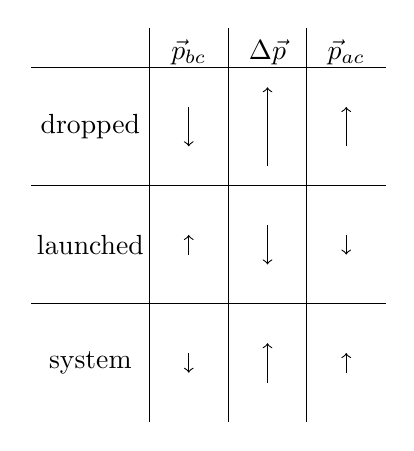
\begin{tikzpicture}
		\node at (0.5,0.7) {$\vec{p}_{bc}$};
		\node at (1.5,0.7) {$\Delta\vec{p}$};
		\node at (2.5,0.7) {$\vec{p}_{ac}$};
		\node at (-0.75,-0.25) {dropped};
		\node at (-0.75,-1.75) {launched};
		\node at (-0.75,-3.25) {system};
		\draw (-1.5,0.5) -- (3,0.5);
		\draw (-1.5,-1) -- (3,-1);
		\draw (-1.5,-2.5) -- (3,-2.5);
		\draw (0,1) -- (0,-4);
		\draw (1,1) -- (1,-4);
		\draw (2,1) -- (2,-4);
		\draw[->] (0.5,0) -- (0.5,-0.5);
		\draw[->] (1.5,-0.75) -- (1.5,0.25);
		\draw[->] (2.5,-0.5) -- (2.5,0);
		\draw[->] (0.5,-1.875) -- (0.5,-1.625);
		\draw[->] (1.5,-1.5) -- (1.5,-2);
		\draw[->] (2.5,-1.625) -- (2.5,-1.875);
		\draw[->] (0.5,-3.125) -- (0.5,-3.375);
		\draw[->] (1.5,-3.5) -- (1.5,-3);
		\draw[->] (2.5,-3.375) -- (2.5,-3.125);
	\end{tikzpicture}
\end{center}
This situation conserves energy for each ball, but not the momentum of the whole system (as $\Delta\vec{p}_{sys}$ is nonzero). We need the change in momentum for the launched ball to be equal and opposite to the change in momentum of the dropped ball, which requires making the momentum of the launched ball equal in magnitude to the momentum of the dropped ball, as shown in this diagram:
\begin{center}
	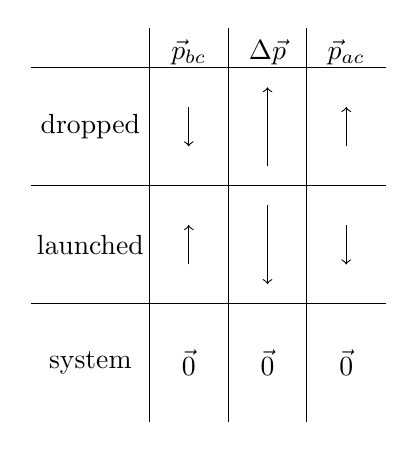
\begin{tikzpicture}
		\node at (0.5,0.7) {$\vec{p}_{bc}$};
		\node at (1.5,0.7) {$\Delta\vec{p}$};
		\node at (2.5,0.7) {$\vec{p}_{ac}$};
		\node at (-0.75,-0.25) {dropped};
		\node at (-0.75,-1.75) {launched};
		\node at (-0.75,-3.25) {system};
		\draw (-1.5,0.5) -- (3,0.5);
		\draw (-1.5,-1) -- (3,-1);
		\draw (-1.5,-2.5) -- (3,-2.5);
		\draw (0,1) -- (0,-4);
		\draw (1,1) -- (1,-4);
		\draw (2,1) -- (2,-4);
		\draw[->] (0.5,0) -- (0.5,-0.5);
		\draw[->] (1.5,-0.75) -- (1.5,0.25);
		\draw[->] (2.5,-0.5) -- (2.5,0);
		\draw[->] (0.5,-2) -- (0.5,-1.5);
		\draw[->] (1.5,-1.25) -- (1.5,-2.25);
		\draw[->] (2.5,-1.5) -- (2.5,-2);
		\node at (0.5,-3.25) {$\vec{0}$};
		\node at (1.5,-3.25) {$\vec{0}$};
		\node at (2.5,-3.25) {$\vec{0}$};
	\end{tikzpicture}
\end{center}

In symbolic form, the change of the momentum of the dropped ball is
\[
\Delta \vec{p}_{d} = \vec{p}_{dac}-\vec{p}_{dbc} = -2\vec{p}_{dbc} = 2p_{dbc}\hat{y},
\]
so by conservation of momentum, it must be that $\Delta\vec{p}_{l} = -2p_{dbc}\hat{y}$. In turn, this means that $\Delta\vec{v}_{l} = -2\frac{p_{dbc}}{m_{l}}\hat{y}$, which gives us
\[
\vec{v}_{lac} = \vec{v}_{lbc} + \Delta\vec{v}_{l} = \left(v_{lbc}-2\frac{p_{dbc}}{m_{l}}\right)\hat{y}.
\]
We need $v_{lbc}-2\frac{p_{dbc}}{m_{l}} = \pm v_{lbc}$ in order to conserve kinetic energy, and $v_{lbc}-2\frac{p_{dbc}}{m_{l}} = v_{lbc}$ would only be possible if $p_{dbc}=0$, which we know is not true, so $\vec{v}_{lac}=-\vec{v}_{lbc}$ (this is another line of reasoning to conclude that the launched ball bounces back from the collision, which we already figured out). In turn, this implies that $\frac{p_{dbc}}{m_{l}} = v_{lbc}$, and therefore
\[
v_{lbc} = \frac{m_{d}}{m_{l}}v_{dbc} = \frac{m_{d}}{m_{l}}\frac{gh}{v_{li}}.
\]
From Eqn. \ref{vcol}, we can see that
\[
\begin{split}
	v_{li}-\frac{gh}{v_{li}} & = \frac{m_{d}}{m_{l}}\frac{gh}{v_{li}} \\
	\implies v_{li} & = \left(\frac{m_{d}}{m_{l}}+1\right)\frac{gh}{v_{li}} \\
	\implies v_{li} & = \sqrt{\left(\frac{m_{d}}{m_{l}}+1\right)gh}.
\end{split}
\]

We can see that $v_{li}$ increases as $m_{d},\ g$, or $h$ increases, which makes sense, as a more massive dropped ball, stronger gravity, or a longer fall all give the dropped ball more momentum right before the collision, which means we have to increase the momentum of the launched ball to successfully turn the dropped ball around. Conversely, $v_{li}$ decreases as $m_{l}$ increases, as we can get the same momentum for less speed by using a more massive ball.

In the special case $m_{l}\gg m_{d}$, that the launched ball is far more massive than the dropped ball, we have $v_{li} \approx \sqrt{gh}$. Note that Eqn. \ref{vcol} tells us that $v_{lbc}\approx\sqrt{gh}-\frac{gh}{\sqrt{gh}}=0$, so starting any slower would mean that the launched ball would be moving down at the time of the collision, and starting any faster would mean that it would be moving up. We know that, in the limit of striking a massive, stationary object in a perfectly elastic collision, the incoming object will reflect back at the same speed. However, if the incoming object were to strike a massive object that was moving, the reflection speed would either be more (for striking an approaching massive object) or less (for striking a receding massive object).

One way to see why involves reasoning in different reference frames; in the frame of an approaching massive object, the incoming object will strike at a speed greater than in a stationary observer's reference frame, and reflect at this greater speed in the massive object's reference frame. In the observer's reference frame, the reflection speed is even larger (as one must add the speed of the massive object's reference frame). Similar reasoning demonstrates the opposite case for the receding massive object.

Anyway, for a massive launched ball, it must be launched at the perfect speed to strike the dropped ball at the instant the massive ball comes to rest, otherwise the launched ball will bounce at the wrong speed.
}